
% ------------ TABLA DE MÉTRICAS FINALES (TEST) ------------
\begin{table}[t]
\centering
\caption{Métricas finales del modelo de Regresión Logística (PyTorch) en el conjunto de prueba.}
\label{tab:metrics-final-pytorch}
\begin{tabular}{lcccc}
\hline
Accuracy & Precision & Recall & F1-Score & ROC AUC \\
\hline
0.725 & 0.760 & 0.704 & 0.731 & 0.805 \\
\hline
\end{tabular}
\end{table}

% ------------ MATRIZ DE CONFUSIÓN ------------
\begin{figure}[t]
\centering
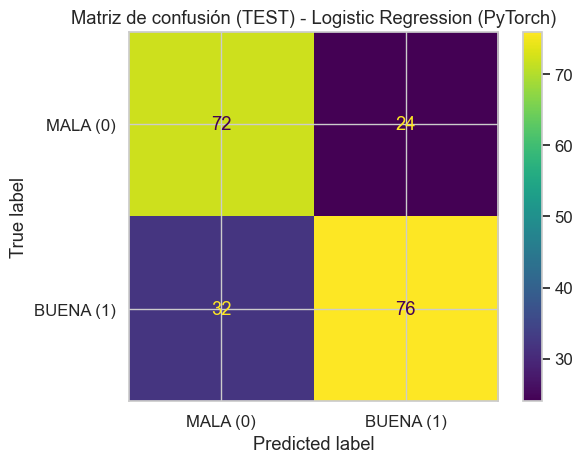
\includegraphics[width=0.75\linewidth]{confusion_matrix_pytorch.png}
\caption{Matriz de confusión en test (MALA=0, BUENA=1).}
\label{fig:cm-final-pytorch}
\end{figure}

% ------------ CURVA ROC ------------
\begin{figure}[t]
\centering
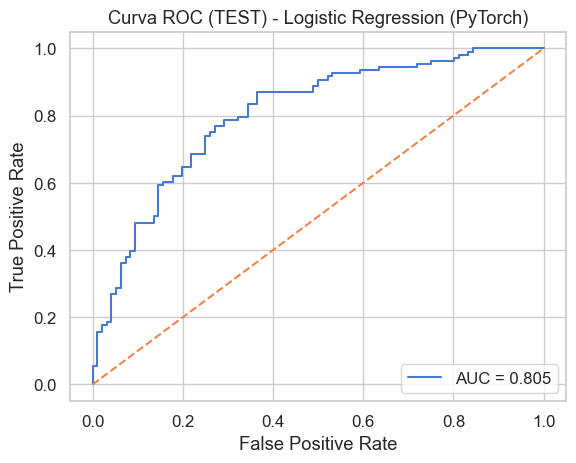
\includegraphics[width=0.75\linewidth]{roc_curve_pytorch.png}
\caption{Curva ROC del modelo en el set de prueba.}
\label{fig:roc-final-pytorch}
\end{figure}
